\documentclass{article}
\usepackage[utf8]{inputenc}
%\usepackage{cite}
\usepackage{graphicx}
\usepackage{listings}
\usepackage{url}

\title{GDMA Project: \\ CDDB as Graph Database}
\author{Julian Schelb (1069967)}
\date{June 2022}

\newcommand{\name}[1]{\texttt{\emph{#1}}}

\begin{document}

\maketitle

\section{Importing Data}

This chapter describes design decisions made to map the relational CDDB database to a graph database. See Jupyter notebook \path{01_Import_Data.ipynb}.

\begin{figure}[ht]
    \centering
    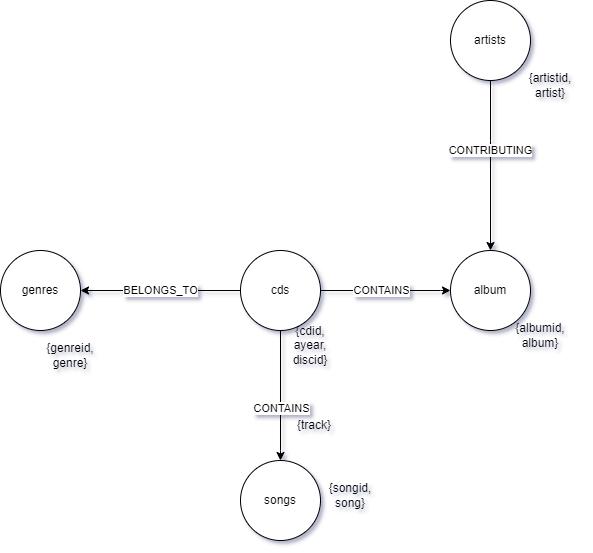
\includegraphics[width=11.5cm]{../Figures/cddb_as_graph-Default.png}
    \caption{CDDB Graph Schema }
\end{figure}

\subsection{Mappping of Tables}
Entries in tables \name{artists}, \name{albums}, \name{songs} and \name{cds} represent entities and are mapped to nodes of appropriate type. The cross table  \name{cdtracks} is mapped as relations between CDs and Songs with the property \name{track}. The cross table  \name{artist2album} is mapped as a triangular relationships, using six relations each to connect Artists, Albums and CDs in both directions.

\subsection{Bidirectional Relations}

To consgtruct the queries necessary for subsequent tasks, it was structly speaking not necessary to create relations for both directions. However, doing so allows for more readable queries. In addition, the relational SQL database does not define a direction for relations either, and this property is thereby preserved.

\subsection{Unique Identifiers}
The unique identifiers present in the SQL database are preserved as node properties. Although Neo4j automatically assigns different IDs internally, this preserves compatibility with the SQL version. It is conceivable that in the real worlds, queries may reference those IDs directly. For example as hardcoded list as part of a GUI.

\subsection{Entity Names}
As in the SQL version, the actual name of a \name{song}, \name{genre}, \name{album} and \name{artist} is a property named after the entity type and therefore different per node label. This was done to map the SQL version as closely as possible to the graph version. In real world scenarios it may be beneficial to rename these properties to \name{name} across all nodes. This would allow for simpler queries in cases where nodes of different types are filtered by name. Also, a joint full-text index would be possible.

\subsection{Indices}
To speed up \texttt{MERGE} and \texttt{MATCH} operations, the IDs for nodes with label \name{Artist}, \name{Album}, \name{Genre}, \name{Song} or \name{CD} are indexed. In addition, a full text index is used for the names of \name{Artists}, \name{Albums} and \name{Songs} to allow for imprecise searches (fuzzy search).

\subsection{Importing Songs}

Songs with a trailing backslashcoused problems because the closing quote is escaped. To mitigate this, an extra whitespace character is added to those song titles. Effected rows can be found with the following sql statement:


\begin{lstlisting}[language=sql]
    SELECT * 
    from cddb.songs s 
    where song like '%\\' 
      and song not like '%\\\\'
\end{lstlisting}

Statement to update the rows:

\begin{lstlisting}[language=sql]
    UPDATE cddb.songs 
    SET song = song || ' ' 
    WHERE song LIKE '%\\' 
      AND song NOT LIKE '%\\\\'
\end{lstlisting}


% Lorem Ipsum ... ~\cite{Nobody06}.

\section{Cypher Queries}

See Jupyter notebook \path{02_Cypher_Queries.ipynb}

\section{SQL to Cypher}

See Jupyter notebook \path{03_SQL_to_Cypher.ipynb}

\section{Searching and Ranking}

See Jupyter notebook \path{05_Searching_Demo.ipynb} for examples search results.

\section{Implementation Details}

This search incorporates nodes corresponding to the input string on the one hand, and the previously liked albums, artists and songs on the other hand. Two separate scores are calculated in a similar manner. Separately calculated Centrality Scores form the basis. Separate graph projections are created for nodes that match the search input and for nodes that have been previously liked. Subsequently, a centrality score is calculated for each node in both. The basic idea is that the most relevant CDs will have a high centrality score. The "Content Match" score and the "User Preference" score are then combined in a weighted manner. The ten CDs with the highest combined score are presented to the user.

\begin{figure}[ht]
    \centering
    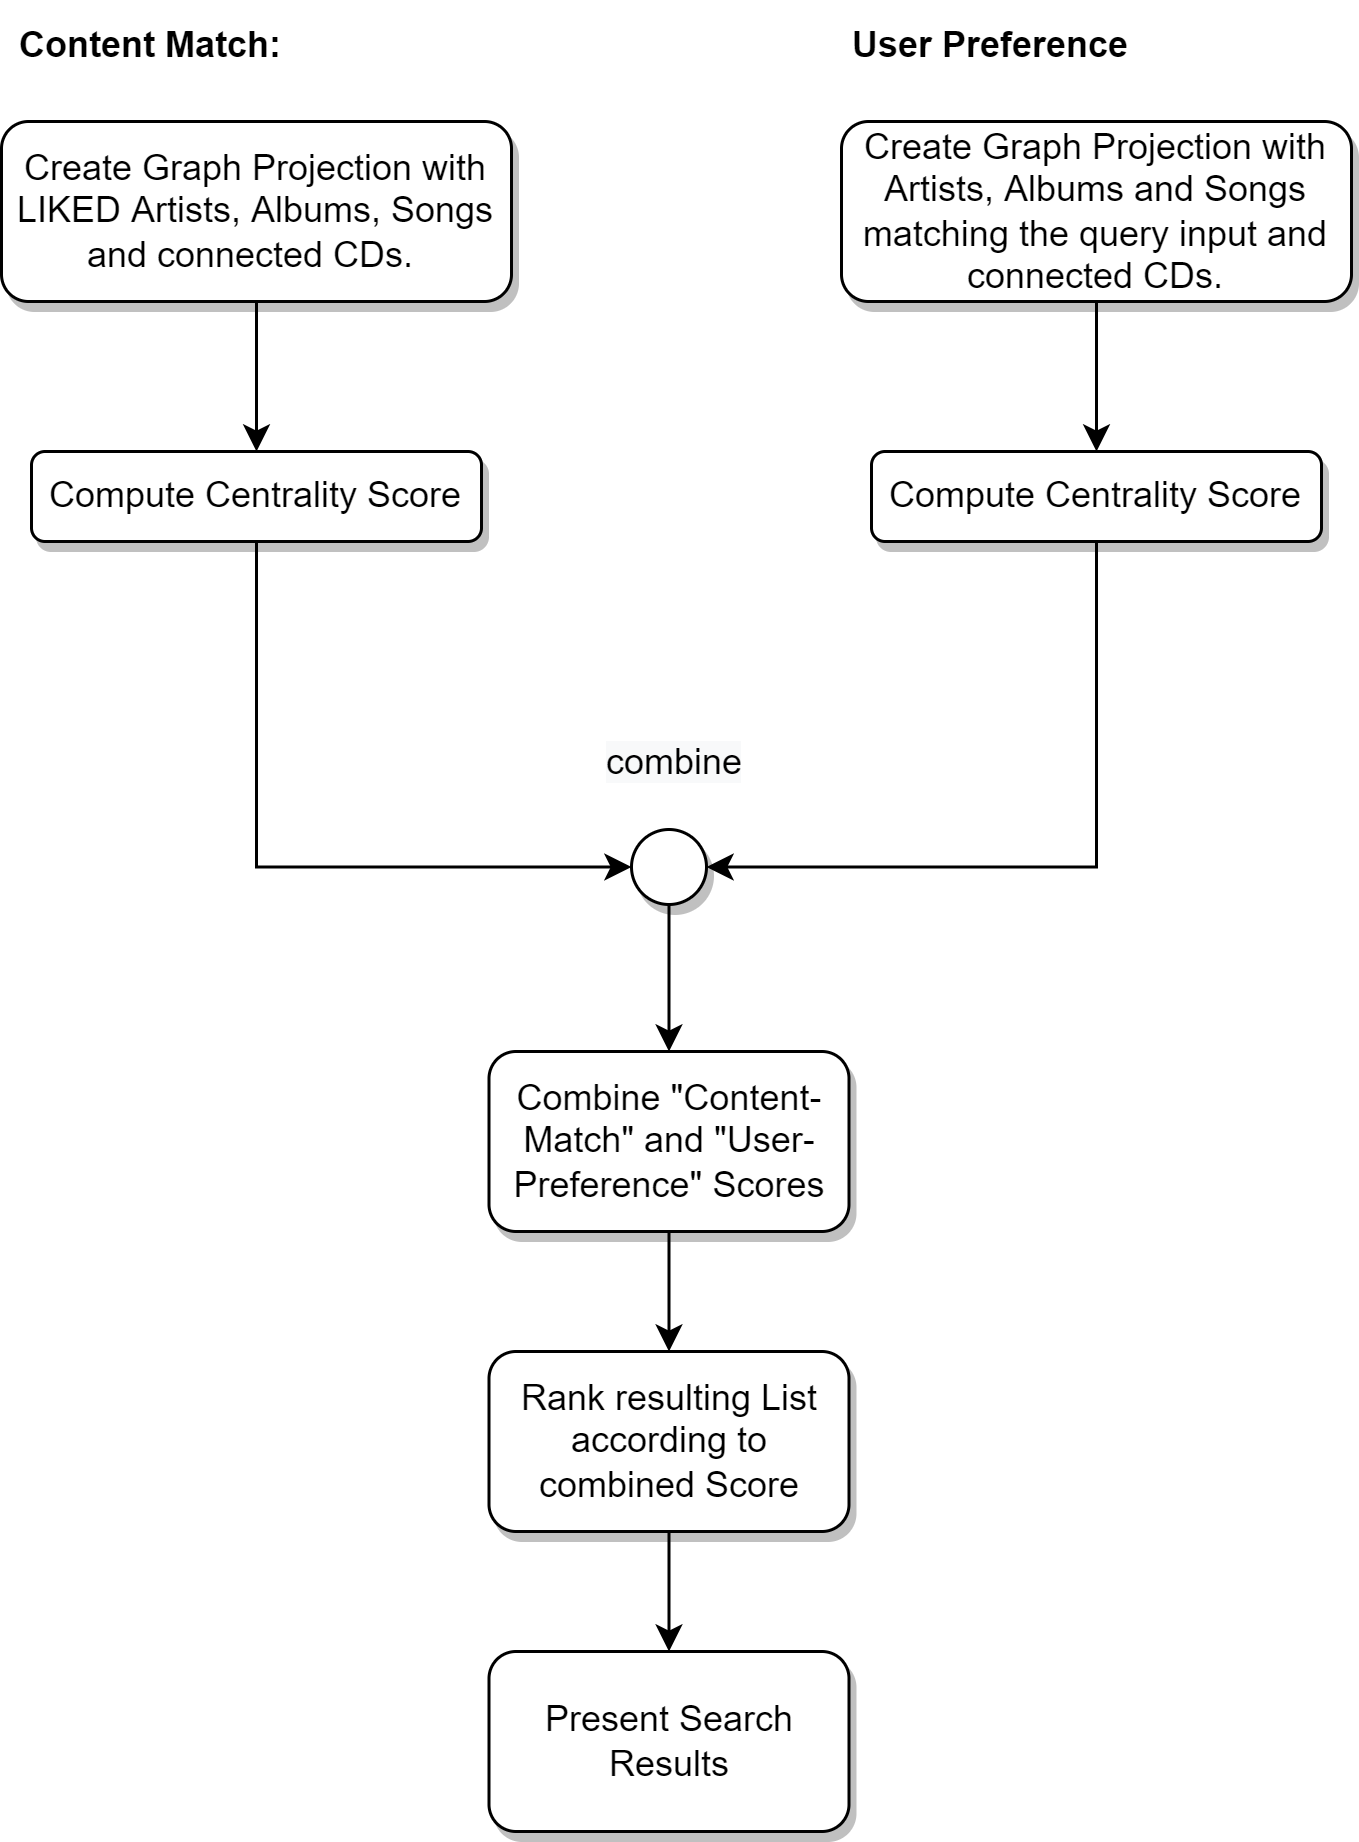
\includegraphics[width=11.5cm]{../Figures/search.png}
    \caption{Process of calculating a "Content Match Score" and a "User Preference Score" to produce a combined result list. }
\end{figure}



% \bibliography{references}{}
% \bibliographystyle{plain}
\end{document}
